%%% The main file. It contains definitions of basic parameters and includes all other parts.

%% Settings for single-side (simplex) printing
% Margins: left 40mm, right 25mm, top and bottom 25mm
% (but beware, LaTeX adds 1in implicitly)
\documentclass[12pt,a4paper]{report}
\setlength\textwidth{145mm}
\setlength\textheight{247mm}
\setlength\oddsidemargin{15mm}
\setlength\evensidemargin{15mm}
\setlength\topmargin{0mm}
\setlength\headsep{0mm}
\setlength\headheight{0mm}
% \openright makes the following text appear on a right-hand page
\let\openright=\clearpage

%% Settings for two-sided (duplex) printing
% \documentclass[12pt,a4paper,twoside,openright]{report}
% \setlength\textwidth{145mm}
% \setlength\textheight{247mm}
% \setlength\oddsidemargin{14.2mm}
% \setlength\evensidemargin{0mm}
% \setlength\topmargin{0mm}
% \setlength\headsep{0mm}
% \setlength\headheight{0mm}
% \let\openright=\cleardoublepage

%% Generate PDF/A-2u
\usepackage[a-2u]{pdfx}

%% Character encoding: usually latin2, cp1250 or utf8:
\usepackage[utf8]{inputenc}

%% Prefer Latin Modern fonts
\usepackage{lmodern}

%% Further useful packages (included in most LaTeX distributions)
\usepackage[titletoc]{appendix}
\usepackage{amsmath}        % extensions for typesetting of math
\usepackage{amssymb}
\usepackage{amsfonts}       % math fonts
\usepackage{amsthm}         % theorems, definitions, etc.
\usepackage{bm}             % boldface symbols (\bm)
\usepackage{graphicx}       % embedding of pictures
\usepackage[numbers]{natbib}         % citation style AUTHOR (YEAR), or AUTHOR [NUMBER]
\usepackage[nottoc]{tocbibind} % makes sure that bibliography and the lists
			    % of figures/tables are included in the table
			    % of contents
\usepackage{dcolumn}        % improved alignment of table columns
\usepackage{booktabs}       % improved horizontal lines in tables
\usepackage{paralist}       % improved enumerate and itemize
\usepackage{xcolor}         % typesetting in color
\usepackage{acronym}		% abbreviations
\usepackage{listings}       % code examples
\usepackage[linesnumbered, boxed, vlined]{algorithm2e}    % algorithms
\usepackage[skip=2pt]{caption}	% captions
\usepackage{makecell}

%%% Basic information on the thesis

% Thesis title in English (exactly as in the formal assignment)
\def\ThesisTitle{Improving Type Inference in the C\# Language}

% Author of the thesis
\def\ThesisAuthor{Tomáš Husák}

% Year when the thesis is submitted
\def\YearSubmitted{2024}

% Name of the department or institute, where the work was officially assigned
% (according to the Organizational Structure of MFF UK in English,
% or a full name of a department outside MFF)
\def\Department{Department of Distributed and Dependable Systems}

% Is it a department (katedra), or an institute (ústav)?
\def\DeptType{Department}

% Thesis supervisor: name, surname and titles
\def\Supervisor{Mgr. Pavel Ježek, Ph.D.}

% Supervisor's department (again according to Organizational structure of MFF)
\def\SupervisorsDepartment{Department of Distributed and Dependable Systems}

% Study programme and specialization
\def\StudyProgramme{Computer Science}
\def\StudyBranch{Software Systems}

% An optional dedication: you can thank whomever you wish (your supervisor,
% consultant, a person who lent the software, etc.)
\def\Dedication{%
\change{Dedication.}
}

% Abstract (recommended length around 80-200 words; this is not a copy of your thesis assignment!)
\def\Abstract{%
\change{Abstract.}
}

% 3 to 5 keywords (recommended), each enclosed in curly braces
\def\Keywords{%
{Type Inference} {C\#} {Roslyn} 
}

%% The hyperref package for clickable links in PDF and also for storing
%% metadata to PDF (including the table of contents).
%% Most settings are pre-set by the pdfx package.
\hypersetup{unicode}
\hypersetup{breaklinks=true}

% Definitions of macros (see description inside)
%%% This file contains definitions of various useful macros and environments %%%
%%% Please add more macros here instead of cluttering other files with them. %%%

%%% Minor tweaks of style

% These macros employ a little dirty trick to convince LaTeX to typeset
% chapter headings sanely, without lots of empty space above them.
% Feel free to ignore.
\makeatletter
\def\@makechapterhead#1{
  {\parindent \z@ \raggedright \normalfont
   \Huge\bfseries \thechapter. #1
   \par\nobreak
   \vskip 20\p@
}}
\def\@makeschapterhead#1{
  {\parindent \z@ \raggedright \normalfont
   \Huge\bfseries #1
   \par\nobreak
   \vskip 20\p@
}}
\makeatother

% This macro defines a chapter, which is not numbered, but is included
% in the table of contents.
\def\chapwithtoc#1{
\chapter*{#1}
\addcontentsline{toc}{chapter}{#1}
}

% Draw black "slugs" whenever a line overflows, so that we can spot it easily.
\overfullrule=1mm

%%% Macros for definitions, theorems, claims, examples, ... (requires amsthm package)

\theoremstyle{plain}
\newtheorem{thm}{Theorem}
\newtheorem{lemma}[thm]{Lemma}
\newtheorem{claim}[thm]{Claim}

\theoremstyle{plain}
\newtheorem{defn}{Definition}

\theoremstyle{remark}
\newtheorem*{cor}{Corollary}
\newtheorem*{rem}{Remark}
\newtheorem*{example}{Example}

%%% An environment for proofs

\newenvironment{myproof}{
  \par\medskip\noindent
  \textit{Proof}.
}{
\newline
\rightline{$\qedsymbol$}
}

%%% An environment for typesetting of program code and input/output
%%% of programs. (Requires the fancyvrb package -- fancy verbatim.)

\DefineVerbatimEnvironment{code}{Verbatim}{fontsize=\small, frame=single}

%%% The field of all real and natural numbers
\newcommand{\R}{\mathbb{R}}
\newcommand{\N}{\mathbb{N}}

%%% Useful operators for statistics and probability
\DeclareMathOperator{\pr}{\textsf{P}}
\DeclareMathOperator{\E}{\textsf{E}\,}
\DeclareMathOperator{\var}{\textrm{var}}
\DeclareMathOperator{\sd}{\textrm{sd}}

%%% Transposition of a vector/matrix
\newcommand{\T}[1]{#1^\top}

%%% Various math goodies
\newcommand{\goto}{\rightarrow}
\newcommand{\gotop}{\stackrel{P}{\longrightarrow}}
\newcommand{\maon}[1]{o(n^{#1})}
\newcommand{\abs}[1]{\left|{#1}\right|}
\newcommand{\dint}{\int_0^\tau\!\!\int_0^\tau}
\newcommand{\isqr}[1]{\frac{1}{\sqrt{#1}}}

%%% Various table goodies
\newcommand{\pulrad}[1]{\raisebox{1.5ex}[0pt]{#1}}
\newcommand{\mc}[1]{\multicolumn{1}{c}{#1}}

%%% User defined macros

%%% Cite
\newcommand{\squarecite}[1]{[\cite{#1}]}

%%% Todo notes
\usepackage{xargs}	% Use more than one optional parameter in a new commands
\usepackage[colorinlistoftodos,prependcaption,textsize=tiny]{todonotes}
\newcommandx{\unsure}[2][1=]{\todo[inline,linecolor=red,backgroundcolor=red!25,bordercolor=red,#1]{#2}}
\newcommandx{\change}[2][1=]{\todo[inline,linecolor=blue,backgroundcolor=blue!25,bordercolor=blue,#1]{TODO: #2}}
\newcommandx{\info}[2][1=]{\todo[inline,linecolor=green,backgroundcolor=green!25,bordercolor=green,#1]{Note: #2}}
\newcommandx{\improvement}[2][1=]{\todo[inline,linecolor=Plum,backgroundcolor=Plum!25,bordercolor=Plum,#1]{#2}}
\newcommandx{\thiswillnotshow}[2][1=]{\todo[inline,disable,#1]{#2}}


% Title page and various mandatory informational pages
\begin{document}
%%% Title page of the thesis and other mandatory pages

%%% Title page of the thesis

\pagestyle{empty}
\hypersetup{pageanchor=false}
\begin{center}

\centerline{\mbox{
\includegraphics[width=166mm]{../img/logo-en.pdf}}}

\vspace{-8mm}
\vfill

{\bf\Large MASTER THESIS}

\vfill

{\LARGE\ThesisAuthor}

\vspace{15mm}

{\LARGE\bfseries\ThesisTitle}

\vfill

\Department

\vfill

{
\centerline{\vbox{\halign{\hbox to 0.45\hsize{\hfil #}&\hskip 0.5em\parbox[t]{0.45\hsize}{\raggedright #}\cr
Supervisor of the master thesis:&\Supervisor \cr
\noalign{\vspace{2mm}}
Study programme:&\StudyProgramme \cr
\noalign{\vspace{2mm}}
Study branch:&\StudyBranch \cr
}}}}

\vfill

% Zde doplňte rok
Prague \YearSubmitted

\end{center}

\newpage

%%% Here should be a bound sheet included -- a signed copy of the "master
%%% thesis assignment". This assignment is NOT a part of the electronic
%%% version of the thesis. DO NOT SCAN.

%%% A page with a solemn declaration to the master thesis

\openright
\hypersetup{pageanchor=true}
\pagestyle{plain}
\pagenumbering{roman}
\vglue 0pt plus 1fill

\noindent
I declare that I carried out this master thesis independently, and only with the cited
sources, literature and other professional sources. It has not been used to obtain another
or the same degree.

\medskip\noindent
I understand that my work relates to the rights and obligations under the Act No.~121/2000 Sb.,
the Copyright Act, as amended, in particular the fact that the Charles
University has the right to conclude a license agreement on the use of this
work as a school work pursuant to Section 60 subsection 1 of the Copyright~Act.

\vspace{10mm}

\hbox{\hbox to 0.5\hsize{%
In \hbox to 6em{\dotfill} date \hbox to 6em{\dotfill}
\hss}\hbox to 0.5\hsize{\dotfill\quad}}
\smallskip
\hbox{\hbox to 0.5\hsize{}\hbox to 0.5\hsize{\hfil Author's signature\hfil}}

\vspace{20mm}
\newpage

%%% Dedication

\openright

\noindent
\Dedication

\newpage

%%% Mandatory information page of the thesis

\openright

\vbox to 0.5\vsize{
\setlength\parindent{0mm}
\setlength\parskip{5mm}

Title:
\ThesisTitle

Author:
\ThesisAuthor

\DeptType:
\Department

Supervisor:
\Supervisor, \SupervisorsDepartment

Abstract:
\Abstract

Keywords:
\Keywords

\vss}

\newpage

\openright
\pagestyle{plain}
\pagenumbering{arabic}
\setcounter{page}{1}


%%% A page with automatically generated table of contents of the master thesis

\tableofcontents

%%% Each chapter is kept in a separate file
\chapter{Introduction}

C\# is an object-oriented programming language developed by Microsoft. 
It belongs to the strongly typed languages helping programmers to possibly reveal bugs at compile time. 
The first part of this thesis focuses on exploring type systems of strongly typed languages and proposes an improvement to the C\# type system. 
The second part concerns the implementation of the improvement in the current C\# compiler and the creation of a proposal that has sufficient potential to be discussed by the \ac{LDM} accepting new C\# language features.

\section{Improving C\# type system}

A key feature of strongly typed languages is type safety, prohibiting operations on incompatible data, achieved by determining data types at compile time. 
The easiest way for a compiler to reason about types of variables in the code is by providing type annotations determining the data type that these variables hold. 
There is Figure \ref{img01:csharp_type_sef} showing an usage of type annotations given by a programmer written in the C\# programming language. 
The type declaration of the \texttt{people} variable guarantees that the following atempt to concatanate \texttt{"Tom"} string to that variable will be reported as an error at compile time since the operation is not defined for a pair of the \texttt{List<string>} type and \texttt{string} type.
\begin{figure}[h]
\begin{lstlisting}[style=csharp]
List<string> people = new List<string>() {"Joe", "Nick"};
people += "Tom"; // Error reported during compilation
\end{lstlisting}
\caption{Type safety in the C\# programming language.}
\label{img01:csharp_type_sef}
\end{figure}
\par
On the other hand, the programmer has to write more code to annotate the variable declaration and object creation whose type has a long name, as we can see in the example. 
This disadvantage of strongly typed languages can be removed by \textit{type inference} when a missing type annotation can be deduced using the context. 
Taking the example shown above, one of the \texttt{List<string>} type annotations could be removed since the type of \texttt{people} variable declaration can be deduced from its initializing value or the type of object creation can be deduced from the type of the assigning variable.
There is an example of C\# type inference in Figure \ref{img02:csharp_type_inf}, where the \texttt{var} keyword is used to trigger type inference determining a type of \texttt{people} variable to be the \texttt{List<string>} type.
\begin{figure}[h]
\begin{lstlisting}[style=csharp]
var people = new List<string>();
\end{lstlisting}
\caption{Type inference in the C\# programming language.}
\label{img02:csharp_type_inf}
\end{figure}
\par
Power of type inference varies in strongly typed languages.
An example of the difference can be seen in type arguments deduction of generic methods. 
In the context of C\#, a generic method is a method that is parametrized by types besides common parameters, as can found in Figure \ref{img03:csharp_gen_meth}.
There is a generic method \texttt{GetField} enabling to return a value of \texttt{o}'s field with the \texttt{fieldName} name.
The type of returned value is generic parameter \texttt{T} since it depends on the type of object's field.
The \texttt{name} variable is initialized by using the method to retrive \texttt{person}'s name which is supposed to be a string.
There is a redundancy in that statement since the type argument list of \texttt{GetField} method could be removed and \texttt{T} could be deduced from the type of \texttt{name} variable which has to be compatible with the return type.
Although, the current version of C\# type inference fails to deduce it.
\begin{figure}
\begin{lstlisting}[style=csharp]
T GetField<T>(object o, string fieldName) { ... }

object person = ...
string name = GetField<string>(person, "name");
\end{lstlisting}
\caption{C\# Type inference of generic methods.}
\label{img03:csharp_gen_meth}
\end{figure}
\par
The similar concept of generic methods were introduced in the Rust \cite{online:rust} programming language which belongs to strongly type languages too.
Figure \ref{img04:rust_gen_meth} shows a definition of generic method \texttt{GetField} which is equivalent of C\# method mentioned in the previous example.
There is equivalent initialization of \texttt{name} variable declaration starting with \texttt{let} keyword, where Rust type inference deduces the type argument \texttt{T} to be \texttt{\&str} type utilizing the type information from the \texttt{name} variable.
\begin{figure}[h]
\begin{lstlisting}[style=csharp]
fn GetField<T>(o: &object, fieldName: &str) -> T { ... }

let person: &object = ...;
let name: &str = GetField(person, "name");
\end{lstlisting}
\caption{Rust Type inference of generic methods.}
\label{img04:rust_gen_meth}
\end{figure}
\par
Although Rust is younger than C\# and has different type system it managed to make type inference more powerful in the context of strongly typed languages to significantly save type annotations typing.
The first goal of this thesis is to investigate if the same level of type inference can be achieved in C\# and improve C\# type inference to be used in more scenarios saving type annotations typing.
\par
The investigation recognizes type system requirements and type inference differencies to achieve desired level of type inference by formalizing Rust and C\# type inference.
These formalizations can be partially identified as a part of existing Hindley-Millner \cite{online:yHM} type inference formalization which helps to unify the processes in these languages.
Traditional Hindley-Millner type inference is defined in the Hindley-Millner type system \cite{online:wikiHM}, where it can deduce types of all variables in an entirely untyped code. 
The power of type inference is caused by properties of the type system, which, in comparison with the C\# type system, doesn't use type inheritance or overloading. 
Despite these barriers, Hindley-Millner type inference can be modified to work with other type systems like Rust or C\#, causing limited use cases where it can be applied.

\section{Implementation}

\info{Describe proposing a new feature}
C\# is an open-source project where the community can contribute by fixing issues of the compiler, proposing new language features, and elaborating on implementing them. 
Proposing new C\# features is done in public discussions of the C\# language repository \cite{online:langRepo}, where everyone can add his ideas or comment on others' ideas. 
Although there is no required structure for how the idea should be described, \ac{LDM} created a template \cite{online:proposalTemplate} containing a base structure for proposing the feature in order to make the idea more likely to be discussed by the team. 
The template includes motivation, detailed description, needed C\# language specification \cite{online:langSpec} changes, and other possible alternatives.
\par
\info{Roslyn}
Language feature prototypes are implemented in feature branches of the Roslyn repository \cite{online:roslynRepo}, which contains an open-source C\# compiler developed by Microsoft and the community.
\par
\info{Present goal of the second thesis part}
The process of language proposal ends with \ac{LDM} accepting or declining it. 
The second part of this thesis regards creating the proposal describing our improvement using the prepared template and implementing it in Roslyn’s feature branch.
\par

\section{Summary}

\info{Goals of this thesis}
We summarize goals of this thesis in the following list:

\begin{enumerate}
  \item[G1.] Explore possibilities of type inference in strongly typed languages
  \item[G2.] Improve C\# type inference based on previous analysis
  \item[G3.] Create an proposal containing the improvement
  \item[G4.] Implement the prototype in Roslyn
\end{enumerate}
\chapter{C\# programming language}

Introduction \ref{sect01:imprv} presented the programming language C\# and its possible improvement of type inference. 
This chapter continues by describing relevant sections of the C\# language and its type inference algorithm to understand the possible barriers to implement improved type inference. 
Since type inference is a complicated process touching many areas of the C\# language, it firstly sorts these areas into separated groups described in necessary detail to understand all parts of the current type inference. 
These areas concern the C\# type system, including generics and language constructs where the type inference occurs or interacts with.

\section{Type system}

\begin{figure}[b]
\centering
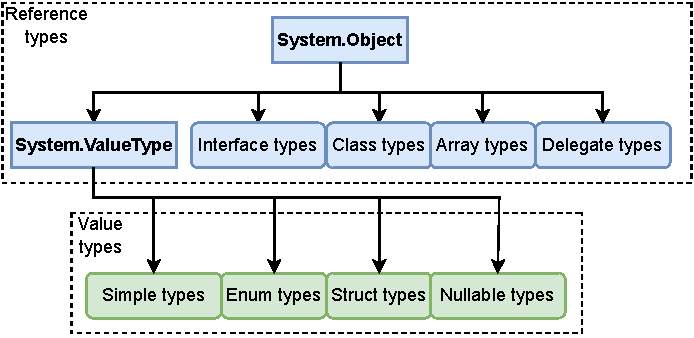
\includegraphics[width=140mm, height=65mm]{./img/CSTypeSystem.pdf}
\caption{The C\# data types schema adjusted from a C\# blog\cite{online:cSharpTypeSystem}.}
\label{img04:typeSys}
\end{figure}
C\# data types are defined in the C\# type system, which also defines relations between them. 
The most fundamental relation is type inheritance, where every type inherits another type, forming a tree with \texttt{System.Object} as a root node that doesn’t inherit any type.
Types are divided into value and reference types, shown in Figure \ref{img04:typeSys}, where an arrow means \textit{is inherited by} relation. 
Value types consist of built-in numeric types referred to as \textit{simple types}, and enumerations referred to as \textit{enum types}, structures referred to as \textit{struct types}, and nullable types. 
Compared to reference types, value types are implicitly sealed, meaning that they can’t be inherited by other types. 
Reference types consist of interfaces, classes, arrays, and delegates. 
An interface introduces a new relation to the type system by defining a list of methods, called a contract, which has to be implemented by a type that implements the interface.
The relation forms an acyclic graph, meaning a type can implement multiple interfaces, but the implementation relations can’t form a cycle. 
Delegates represent typed pointers to methods describing its signature, including generic parameters, parameters, and a return type.
\par
The type system implicitly allows to assign \texttt{null}, indicating an invalid value, to reference types. Since C\# 2.0 \cite{online:csHist}, it allows to assign \texttt{null} value to nullable types, which are equivalents of the rest of value types prohibiting it. Because assigning \texttt{null} value is referred to as a billion-dollar mistake \cite{online:billionDolarMistake}, C\# 8.0 \cite{online:csHist}, introduced optional settings warning about assigning null values and created nullable reference types, which, together with nullable types, explicitly allows \texttt{null} assignment as a way of interaction with legacy code not using the feature.
\par
A big part of the type system is C\# \textit{generics}, allowing the parameterization of types and methods by arbitrary types. 
A specific generic method or type is \textit{constructed} by providing required type arguments, where \textit{construction} means replacing all occurrences of type parameters with the type arguments. 
Since type argument can be arbitrary type, the type parameter is considered to be the most general type in the type system, \texttt{System.Object}. 
Assuming additional API from the type parameter is achieved by restricting a set of types, which can replace the type parameter, enabling a specific interface of this set. 
The restriction is described by type constraints, which can be applied to type parameters. 
There are several kinds of constraints that can be combined together, forcing the type argument to fulfill all of them. 
Figure \ref{img05:typeConst} shows only two of them, and the rest can be found in the C\# documentation \cite{online:csharpTypeConst}. 
There is a definition of the \texttt{PrioritySorter} generic class with the \texttt{TItem} type parameter containing two constraints that the type argument has to hold. 
The \texttt{class} constraint allows only reference types. 
The \texttt{IPriorityGetter} constraint allows only types that implement the
interface.
\begin{figure}[h]
\begin{lstlisting}[style=csharp]
class PrioritySorter<TItem> where TItem : class, IPriorityGetter 
{ ... }
\end{lstlisting}
\caption{C\# type constraints.}
\label{img05:typeConst}
\end{figure}
\par
Constructed methods and types are new entities that don’t have any special relations between themselves implied from the construction. 
However, C\# generic interfaces can utilize a concept of type variance to introduce additional relations between constructed types. 
Initially, type parameters are \textit{invariant}, meaning an obligation to use the same type arguments as initially required. 
A type parameter can be specified to be \textit{covariant}, by prepending the type parameter declaration with the \texttt{in} keyword, allowing to use more derived type than initially required. 
0pposite \textit{contravariance} uses the \texttt{out} keyword, allowing to use
more general type than initially required.
\par
The last relevant feature of the type system is method overloading, which
allows definitions of multiple methods with the same name, return type, and count of type parameters having different types of parameters. 
Further chapters will mention the feature as an obstacle in designing efficient type inference.

\section{Relevant constructs}

Many unrelated C\# constructs can use type inference or can influence the type inference algorithm.
There are the most relevant whose internals are then considered in the following chapters regarding the design of the improvement.

\subsection*{Dynamic}

Introduction \ref{sect01:imprv} mentioned that strongly typed languages require knowing data types at compile time to prohibit incompatible operations on them. 
In the context of C\#, data means values of expressions that are transformed by operations defined on their types. 
It turned out that operations on expressions of unknown type at compile time became crucial for interoperability with other dynamic-typed languages whose types of expressions are known at runtime. 
To make the interoperability easier, C\# introduced the \texttt{dynamic} type that can be used as an ordinary type, which avoids the checks and causes \textit{dynamic binding}. 
\textit{Binding} is a process of resolving referenced operations based on the type and value of the expression. 
The majority of the C\# binding happens statically at compile time. Expressions containing a value of the \texttt{dynamic} type are dynamic bound at runtime, bypassing the static binding of the compiler. 
This behavior can lead to possible bugs regarding invalid operations on the dynamic data types, which will be reported during runtime. 
Figure \ref{img06:dynamic} shows a declaration of the \texttt{a} variable of the dynamic type.
Dynamic binding occurs in the \texttt{a.Foo()} expression, where the \texttt{Foo()} operation is not checked during compilation. 
An error is reported at runtime when the actual type of the \texttt{a} variable is determined to be \texttt{string}, which doesn’t define \texttt{Foo()} operation. Despite the dynamic binding, a compiler can still little check certain kinds of expressions containing values of dynamic types to reveal possible errors at compile time. 
An example of such checking is the \texttt{Bar()} method call, where the compiler can check the first argument, whose type is known at compile time as the type of the parameter. 
An appropriate error occurs during the compilation because string value has the \texttt{string} type, and it is passed as the \texttt{p1} parameter, which has the \texttt{int} type.
\begin{figure}[h]
\begin{lstlisting}[style=csharp]
void Bar<T>(int p1, T p2, long p3) { ... }
...
dynamic a = "string";
a.Foo();
Bar("string", 1, a); \\ Compilation error reported
\end{lstlisting}
\caption{C\# dynamic type.}
\label{img06:dynamic}
\end{figure}

\subsection*{Anonymous function}

C\# allows to define a function without a name, called \textit{anonymous function}.
The function is represented as an expression that can be called or stored in a variable.
There are three types of anonymous function.
The first type is \textit{anonymous method} shown in Figure \ref{img06:anonymousF} where it is stored in the \texttt{a} variable.
The \texttt{b} variable contains the second type called \textit{explicit typed anonymous function}.
The third variable \texttt{c} contains the last type called \textit{implicit typed anonymous function}.
As can be seen, all of them have inferred return types based on return expression inside their bodies.
The most interesting type is the last one, where even parameter types are inferred based on a surrounding context and which is especially threatened by \textit{method type inference} algorithm mentioned in method type inference section \ref{sect02:MTIA}.
\begin{figure}[h]
\begin{lstlisting}[style=csharp]
Func<int, int> a = delegate(int p1) { return p1 + 1; };
Func<int, int> b = (int p1) => { return p1 + 1; };
Func<int, int> c = (p1) => { return p1 + 1; };
\end{lstlisting}
\caption{C\# anonymous functions.}
\label{img06:anonymousF}
\end{figure}

\subsection*{Object creation expression and initializer}

Initializers are used as a shortcut during an object instantiation.
The simplest one is \textit{object initializer} allowing to assign values to the object's fields pleasantly instead of assigning them separately after the initialization.
The second type of initializers regards arrays and collections.
\textit{Array initializers} are used to create fixed-size arrays with predefined content.
Figure \ref{img07:initializer} shows the \texttt{arrayInit} variable initialized by an array of \texttt{int} with two items using the initializer.
Under the hood, each item in the initializer is assigned to the corresponding index of the array after the array creation.
\textit{Collection initializers} are similar to array initializers defined on collections, which are created by implementing \texttt{ICollection<T>} interface.
One of the interface's declaring methods is \texttt{void Add<T>(T)} with adding semantics.
Each type implementing this interface is allowed to use an initializer list in the same manner as an array initializer.
It's just a sugar code hiding to call the \textit{Add} method for each item in the initializer list.
The last type of an initializer uses an indexer to store referred values on predefined positions, which is used in the second statement where the \texttt{indexerInit} variable is initialized by a dictionary object using indexers in its initializer list.
\begin{figure}[h]
\begin{lstlisting}[style=csharp]
var arrayInit = new int[] { 1, 2 };
var indexerInit = new Dictionary<string, int>() { 
    ["a"] = 1, ["b"] = 2 
};
\end{lstlisting}
\caption{C\# collection initializer.}
\label{img07:initializer}
\end{figure}

\section{Type inference} \label{sect02:typeInference}

C\# type inference occurs in many contexts. 
However, the proposed improvement will be inspired by and influence only a few of them.
These contexts are presented below.

\subsection{Keyword \texttt{var}}
One of the simplest type inference occurrences regards the \texttt{var} keyword used in a variable declaration.
It lets the compiler decide the type of variable based on the type of initializing value, which implies that it can’t use the keyword in declarations without initializing the value.
Figure \ref{img07:var} shows the usage, where the type of the \texttt{a} variable is determined to be \texttt{string} since it is initialized by a string value. 
\begin{figure}[h]
\begin{lstlisting}[style=csharp]
var a = "str";
\end{lstlisting}
\caption{Keyword \texttt{var}.}
\label{img07:var}
\end{figure}

\subsection{Operator \texttt{new()}}

There is also an opposite way of deducting types from a target to a source.
An example is the \texttt{new()} operator, which can be called with arbitrary arguments and represents object creation of a type that is determined by a type of the target. 
An example of these situations can be seen in Figure \ref{img08:new} where the target-typed \texttt{new(1)} operator allows to skip the specification of creating type in the object creation expression since the \texttt{myList} variable type gives it. After the type inference, the operator represents the new \texttt{new List<int>(1)} object creation expression.
\begin{figure}[h]
\begin{lstlisting}[style=csharp]
List<int> myList = new(1);
\end{lstlisting}
\caption{Operator \texttt{new()}.}
\label{img08:new}
\end{figure}

\subsection{Method type inference} \label{sect05:mti}

Method type inference is the most complex C\# type inference used during generic method call binding when type arguments are not given.
Figure \ref{img09:methodTypeInf} shows a situation when the method type inference deduces \texttt{System.String}, \texttt{System.Int32} and \texttt{System.Int32} as type arguments of the \texttt{Foo} method. 
There is a multi-step process that the type inference has to do to be able to infer it. 
Regarding the \texttt{T1} type parameter, the inference has to find a common type between the \texttt{(long)1} argument and the \texttt{(int)1} argument. 
Regarding the \texttt{T2} type parameter, the type inference has to go into type arguments of the generic type of the \texttt{p3} parameter and the \texttt{myList} argument, check if the types are compatible, and then match the \texttt{T2} type parameter against the \texttt{int} type argument of the \texttt{List<int>}. 
The \texttt{T3} type parameter is the most challenging since it occurs as a return type of the delegate. 
The type inference has first to infer types of input parameters of this delegate to be able to infer the implicit anonymous function’s return type. 
Then, it can match the inferred return type with the \texttt{T3} type parameter, resulting in the \texttt{System.Int32} type.
\begin{figure}[h]
\begin{lstlisting}[style=csharp]
Foo<T1, T2, T3>(T1 p1, T1 p2, IList<T2> p3, Func<T2, T3> p4)
{ ... }
...
List<int> myList = ...
Foo((long)1, (int)1, myList, (p1) => p1 + 1);
\end{lstlisting}
\caption{Method type inference.}
\label{img09:methodTypeInf}
\end{figure}
\par
The method type inference algorithm is detailly described in separate section \ref{sect02:MTIA} since it is a complex algorithm, and the proposed improvement will be based on that.

\subsection{Array type inference}

The last mentioned type inference happens in array initializers when the array type should be deduced from the initializer list. 
Figure \ref{img14:arrayTypeInf} shows an example of a situation when the type inference is used for determining the element type of the constructing array. 
The C\# specification calls it \textit{common type inference}, which finds the most specialized common type between given types.
In this case, it is the \texttt{object} type.
From one point of view, it is just adjusted the method type inference algorithm where there is just one type variable, and all initializer items are lower bounds of that type variable.
\begin{figure}[h]
\begin{lstlisting}[style=csharp]
new[] { new object(), "string" };
\end{lstlisting}
\caption{Array type inference.}
\label{img14:arrayTypeInf}
\end{figure}

\section{Method type inference algorithm} \label{sect02:MTIA}

Since one of the thesis's improvements is adjusting the method type inference algorithm, this section presents
its description. 
The thesis doesn’t show the complete algorithm described in the C\# specification \cite{online:csTypeInference} since it is complex, and some parts are unimportant for the following chapters. 
The simplified algorithm is divided into four subsections. 
The algorithm uses several definitions presented below.
\begin{defn}[Fixed type variables, bounds]
We call inferred type parameters \emph{type variables} which are at the beginning of the algorithm unknown, \emph{unfixed}. 
During the algorithm, they start to be restricted by sets of type \emph{bounds}.
The type variable becomes \emph{fixed} when the its actual type is determined using its \emph{bounds}.
\end{defn}
\begin{defn}[Method group]
A \emph{method group} is a set of overloaded methods resulting from a member lookup.
\end{defn}
\begin{defn}[Input/Output types]
If \texttt{E} is a method group or anonymous function and \texttt{T} is a delegate or expression tree type, then return type of \texttt{T} is an \emph{output type} of \texttt{E}.
If \texttt{E} is a method group or implicitly typed anonymous function, then all the parameter types of \texttt{T} are \emph{input types} of \texttt{E}. 
\end{defn}
\begin{defn}[Dependence]
An unfixed type variable \texttt{$X_i$} \emph{depends directly on} an unfixed type variable \texttt{$X_e$} if for some argument \texttt{E} \texttt{$X_e$} occurs in an input type of \texttt{E} and \texttt{$X_i$} occurs in an output type of \texttt{E}.
\texttt{$X_i$} \emph{depends on} \texttt{$X_e$} is the transitive but not reflexive closure of \emph{depends directly on}.
\end{defn}
\begin{table}[h]
\begin{center}
\begin{tabular}{ | l | l | } 
  \hline
  \texttt{\{Parameter\}.isValParam} & \makecell[lc]{Checks if the parameter is passed by\\ value.}\\ 
  \hline
  \texttt{\{Parameter\}.isRefParam} & \makecell[lc]{Checks if the parameter is passed by\\ reference.} \\ 
  \hline
  \texttt{\{Parameter\}.isOutParam} &\makecell[lc]{ Checks if the parameter has\\ \texttt{out} modifier.}\\ 
  \hline
  \texttt{\{Parameter\}.isInParam} & \makecell[lc]{Checks if the parameter has\\ \texttt{in} modifier.}\\ 
  \hline
  \texttt{\{Argument\}.isInArg} & \makecell[lc]{Checks if the argument has\\ \texttt{in} modifier.}\\ 
  \hline
  \texttt{\{Type\}.outTypes} & Returns \textit{Output} types of type.\\ 
  \hline
  \texttt{\{Type\}.inTypes} & Returns \textit{Input} types of type.\\ 
  \hline
  \texttt{\{Type\} isLike '\{Pattern\}'} & \makecell[lc]{Checks if the type matches\\ the pattern.}\\ 
  \hline
  \texttt{\{Type\}.isDelegateOrExprTreeType} & \makecell[lc]{Checks if the type is Delegate\\ or Expression Tree type.}\\ 
  \hline
\end{tabular}
\end{center}
\caption{Description of used properties.}
\label{table1:algorithmLegen}
\end{table}
\par
The pseudocode describing the algorithm uses custom helper functions explained in Table \ref{table1:algorithmLegen}.

\subsection{Algorithm phases}

Figure \ref{img10:methodTypeInference1} shows the initial phases of the algorithm. 
The method type inference process starts with receiving arguments of a method call and the method’s signature, which type parameters have to be deduced. 
The algorithm has two phases, where the first phase initializes initial bounds’ sets of type variables (inferred type arguments), and the second phase repeats until all type variables are fixed or fail if there is insufficient information to deduce them. 
Each type variable has three types of bounds. 
The exact bound consists of types, which have to be identical to the type variable, meaning that they can be converted to each other. 
The lower bound contains types that have to be convertible to the type variable, and the upper bound is opposite to it.
\begin{figure}[h!]
\begin{lstlisting}[style=myAlgo, mathescape=true]
Input: method call M($E_1$,...$E_x$) and 
       its signature $T_e$ M<$X_1$,...,$X_n$>($T_1$ $p_1$,...,$T_x$ $p_x$)
Output: inferred $X_1$,...$X_n$
  $B_{lower}$ = $B_{upper}$ = $B_{exact}$ = F = []
  FirstPhase()
  SecondPhase()

fn FirstPhase():
  E.foreach(e $\rightarrow$  
    if (e.isAnonymousFunc)
      InferExplicitParamterType(e, $T$[e.idx])
    elif (e.getType() is Type u)
      switch (u) {
        p[e.idx].isValParam $\rightarrow$ InferLowerBound(u, $T$[e.idx])
        p[e.idx].isRefParam || p[e.idx].isOutParam $\rightarrow$ 
          InferExact(u, $T$[e.idx])
        p[e.idx].isInParam && e.isInArg $\rightarrow$ 
          InferLowerBound(u, $T$[e.idx])
      }
  )
  
fn SecondPhase():
  while (true):
    $X_{indep}$ = $X$.filter(x $\rightarrow$ 
      F[x.idx] == null && $X$.any(x $\rightarrow$ dependsOn(x, y)))
    $X_{dep}$ = $X$.filter(x $\rightarrow$
      F[x.idx] == null && $X$.any(y $\rightarrow$ 
        dependsOn(y, x) && ($B_{lower}$+$B_{upper}$+$B_{exact}$).isNotEmpty))
    switch {
	  $X_{indep}$.isNotEmpty $\rightarrow$ $X_{indep}$.foreach(x $\rightarrow$ Fix(x))     
	  $X_{dep}$.isNotEmpty && $X_{indep}$.isEmpty $\rightarrow$ $X_{dep}$.foreach(x $\rightarrow$ Fix(x))
	  ($X_{indep}$+$X_{dep}$).isEmpty $\rightarrow$ 
	    return if (F.any(x $\rightarrow$ x == null)) Fail() else Success(F)
	  default $\rightarrow$ $E$.filter(e $\rightarrow$ 
	      $X$.any(x $\rightarrow$ 
	        F[x.idx] == null && $T$[e.idx].outTypes.contains(x)) 
	      && !X.any(x $\rightarrow$ 
	        F[x.idx] == null && $T$[e.idx].inTypes.contains(x))
	    ).foreach(e $\rightarrow$ InferOutputType(e, $T$[e.idx]))
    }
\end{lstlisting}
\caption{Phases of Method Type Inference}
\label{img10:methodTypeInference1}
\end{figure}
\par
\texttt{FirstPhase()} iterates over provided arguments and matches their types with types of corresponding parameters. 
This matching has two goals. 
The first is to check the compatibility of matched types, and the second is to collect the mentioned bounds associated with type variables contained in parameters’ types. 
This matching has many rules, followed by helping functions mentioned later in this section.
The matching represents dealing with the \texttt{T2} type parameter mentioned in Figure \ref{img09:methodTypeInf} where the compatibility between \texttt{List<int>} and \texttt{IList<T2>} is firstly checked, and then the \texttt{int} type is added as a lower bound of the \texttt{T2} type parameter. 
Type variables can have dependencies between themselves, so the first phase postpones matching output types of arguments’ types with corresponding parameters’ types because the output types can contain dependent type variables.
\par
\texttt{SecondPhase()} happens iteratively, respecting the \textit{depends on} relation.
Each iteration has two goals.
The first one is the fixation of at least one type variable.
If there is no type variable to fix because either all type variables are fixed or there are no other type bounds that could be used for type variable deduction, the algorithm ends.
The sets \texttt{$X_{indep}$} and \texttt{$X_{dep}$} refer to type variables, which can be fixed in the current iteration.
Line 31 contains the ending condition of the algorithm when all type variables are fixed, or there is no way to infer the next ones.
The second goal is to match postponed matching of output types of arguments' types with output types of corresponding parameters' types where all type variables in the output type of a parameter type don't depend on unfixed variable types contained in input types of the parameter type.
The second goal is to match postponed matching of output types of arguments' types with output types of corresponding parameters' types where all type variables in the output type of a parameter type don't depend on unfixed variable types contained in input types of the parameter type.
Line 32 describes this process using the pseudocode.
This goal represents dealing with implicit anonymous functions mentioned in Figure \ref{img09:methodTypeInf} where \texttt{T3} depends on \texttt{T2}.
The algorithm first infers the \texttt{T2} input type of the anonymous function, then infers the function's output type, which is then used to match the output type of \texttt{Func<T2, T3>} parameter type with the output type of the inferred anonymous function's type.
The match yields the \texttt{int} upper bound of the \texttt{T3} type parameter.

\subsection{Function type inference}

Figure \ref{img11:methodTypeInference2} contains definitions of two helper functions used in the first and second phases. 
The \texttt{ExplicitParameterType()} function is used to match an argument type, which is an explicit typed anonymous function. 
This function has typed parameters, so the algorithm matches them with input types of the corresponding parameter type.
\par
The \texttt{InferOutputType()} function is used in the second phase when postponed
matching of output types happens. 
Because potential type variables contained in the return types don’t depend on any unfixed type variables, the algorithm can match them. 
There are two situations where the output type is matched. 
The first situation regards anonymous functions, where the algorithm first infers the return type represented by the \texttt{InferReturnType()} function and then matches it with the output type of the corresponding parameter. 
The second situation regards method groups, which are firstly resolved by \texttt{OverloadResolution()}. 
The return type of the resolved method is matched with the output type of the corresponding parameter.
\begin{figure}[h!]
\begin{lstlisting}[style=myAlgo, mathescape=true]
fn InferExplicitParameterType(Argument E, Type T):
  if (E.isExplicitTypedAnonymousFunc && T.isDelegateOrExprTreeType
    && E.paramTypes.size == T.paramTypes.size)
      E.paramTypes.zip(T.paramTypes)
                  .foreach((e, t) $\rightarrow$ InferExact(e, t))
fn InferOutputType(Argument E, Type T):
  switch(E) {
	E.isAnonymousFunc && $T$.isDelegateOrExprTreeType $\rightarrow$
	  InferLower(InferReturnType(E), T.returnType) 
	E.isMethodGroup && T.isDelegateOrExprTreeType $\rightarrow$ {
	  	$E_{resolved}$= OverloadResolution(E, T.parameterTypes)
	  	if ($E_{resolved}$.size == 1) 
	  	  InferLower($E_{resolved}$[0].returnType, T.returnType) 
	  }
	E.isExpression && E.getType() is Type u $\rightarrow$ InferLower(u, T)
  }
\end{lstlisting}
\caption{\textit{Explicit parameter type inference}, \textit{Output type inference}}
\label{img11:methodTypeInference2}
\end{figure}
\newpage
\subsection{Collecting Type bounds}

Figure \ref{img12:methodTypeInference3} shows three functions that add new bounds to type variables’
bound sets. 
Basically, all of them have similar behavior. 
It traverses the given \texttt{U} type contained in the argument type with the \texttt{V} type contained in the corresponding parameter type using the conditions contained in the \texttt{switch} statement and adds the \texttt{U} type to the type variable’s bound when the \texttt{V} type is a type variable. 
Since the branching conditions in \texttt{InferLower} and \texttt{InferUpper} are similar to those in \texttt{InferExact} and unimportant for the proposed improvement, the thesis omits it.
\begin{figure}[h!]
\begin{lstlisting}[style=myAlgo, mathescape=true]
fn InferExact(Type U, Type V):
  if (Type t = X.find(x $\rightarrow$ V == x && F[x.idx] == null)) 
    $B_{exact}$[t.idx].add(U)
  switch(V) {
    V isLike '$V_1$[..]' && U isLike '$U_1$[..]' && V.rank == U.rank $\rightarrow$ 
      InferExact($U_1$, $V_1$)
    V isLike '$V_1$?' && U isLike '$U_1$' $\rightarrow$ InferExact($V_1$, $U_1$)
    V isLike 'C<$V_1,...,V_e$>' && U isLike 'C<$U_1,...,U_e$>' $\rightarrow$
      V.typeArgs.zip(U.typeArgs)
                .foreach((v, u) $\rightarrow$ InferExact(v, u)) 
  }
  
fn InferLower(Type U, Type V):
  if (Type t = X.find(x $\rightarrow$ V == x && F[x.idx] == null)) 
    $B_{lower}[t.idx]$.add(U)
  switch { .... }
  
fn InferUpper(Type U, Type V):
  if (Type t = X.find(x $\rightarrow$ V == x && F[x.idx] == null)) 
    $B_{upper}[t.idx]$.add(U)
  switch { ... }
\end{lstlisting}
\caption{\textit{Exact inference}, \textit{Upper-bound inference}, \textit{Lower-bound inference}}
\label{img12:methodTypeInference3}
\end{figure}
\par
\begin{obs}
There is no need to check possible contradictions because they are checked in the type variable fixation. 
\end{obs}
\begin{obs}
Bound sets don't contain unfixed type variables, which makes the algorithm simpler and which will be important for the following chapters.
The reason for that can be noticed in the design of functions API, where the left parameter always contains an expression or type from the argument, and the right parameter contains a type from the inferring method parameter. 
Since the three last-mentioned functions add only the type from the left parameter to bounds, there can’t be any type variables because argument types don’t contain type variables.
\end{obs}

\subsection{Fixation}

The last part of this algorithm is type variable fixation, shown in Figure \ref{img13:methodTypeInference4}. 
Initially, a set of candidates for the type variable is constructed by collecting all its bounds.
Then, it goes through each bound and removes the candidates who do not satisfy the bound’s restriction. 
If there is more than one candidate left, it tries to find a unique type that is identical to all left candidates. 
The fixation is successful if the candidate is found. 
The type variable is fixed to that type. 
This process can be seen in the initial example \ref{img09:methodTypeInf}, where the \texttt{T1} type variable contains \texttt{long} and \texttt{int} in its lower bound set. 
At the start of this process, both types are candidates. 
However, \texttt{int} is removed because it doesn’t have an implicit conversion to \texttt{long}.
\par
\begin{figure}[h!]
\begin{lstlisting}[style=myAlgo, mathescape=true]
fn Fix(TypeParameter x):
  $U_{candidates}$ = $B_{lower}$[x.idx] + $B_{upper}$[x.idx] + $B_{exact}$[x.idx]
  $B_{exact}$[x.idx].foreach{b $\rightarrow$ 
    $U_{candidates}$.removeAll(u -> !b.isIdenticalTo(u))}
  $B_{lower}$[x.idx].foreach{b $\rightarrow$ 
    $U_{candidates}$.removeAll(u -> !hasImplicitConversion(b, u))}
  $B_{upper}$[x.idx].foreach{b $\rightarrow$ 
    $U_{candidates}$.removeAll(u -> !hasImplicitConversion(u, b))}
  temp = $U_{candidates}$.filter(x $\rightarrow$ $U_{candidates}$.all(y $\rightarrow$ 
    hasImplicitConversion(y, x)))
  if (temp.size == 1) F[i] = temp[0] else Fail()
\end{lstlisting}
\caption{Fixing of type variables}
\label{img13:methodTypeInference4}
\end{figure}
\par
An important observation of the method type inference is an obligation of infering all type arguments of the method.
If the compiler is not able to infer all type arguments, an user has to specify all type arguments.
C\# currently doesn't offer a way how to hint just ambigious type arguments.
\chapter{Related work}

This chapter follows by mentioning related work regarding the current implementation of the C\# compiler and formalizing C\# type inference using Hindley-Milner type inference, which is explored in more detail with references to its modification in Rust and C\# programming languages.
This knowledge will be utilized as a primary source of inspiration for the improvement.
In the end, it mentions relevant C\# language issues presented on the GitHub repository, which will be used later to prioritize the improvement features to make it more likely to be discussed at \ac{LDM} held by \ac{LDT}. 

\section{Roslyn}

The implementation of C\# type inference can be found in the Roslyn compiler, as open-source C\# and VisualBasic compiler developed at the GitHub repository. 
Presented Roslyn’s architecture will help to better understand the context and restrictions that has to be cosidered to plug the improved type inference into the compiler.
Figure \ref{img15:roslynPip} is used to explain the compilation pipeline \cite{online:roslynArchitecture} which consists of four phases highlighted with different colors.
\begin{figure}[h]
\centering
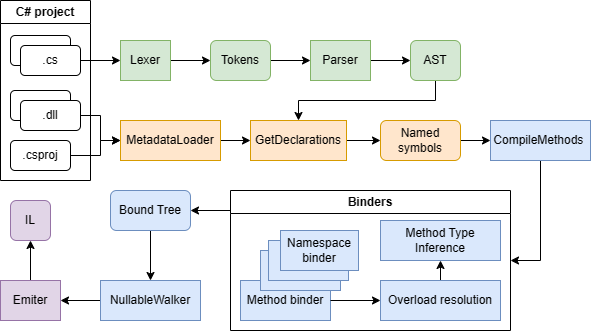
\includegraphics[width=120mm, height=70mm]{./img/Roslyn_Arch.png}
\caption{Roslyn architecture}
\label{img15:roslynPip}
\end{figure}

\subsection{Parsing C\# sources phase}

The pipeline starts with loading the \texttt{.csproj} file with related C\# sources (\texttt{.cs}) and referenced libraries (\texttt{.dll}).
C\# sources are passed to the lexer, creating tokens used by the parser forming \ac{AST}.
\ac{AST} construction is the first phase (green boxes in Figure \ref{img15:roslynPip}) of the compiler checking syntax of C\# sources.

\subsection{Loading named symbols}

The second phase, marked by orange, forms \emph{named symbols} exposed by public API representing defined namespaces, classes, methods, etc., in the C\# project. 
The declarations are received from C\# sources by traversing \as{AST} and seeking for the particular syntax. 
Libraries, stored in \texttt{.dll} format are parsed by \texttt{MetadataLoader}, creating the same named symbols as those received from C\# sources.

\subsection{Binding phase}

The third phase (represented by blue boxes), also called the binding phase, matches identifiers in the code with received named symbols from the previous phase. 
Because the processing of a method body is not dependent on other method bodies since the code only uses already known declarations, Roslyn makes this phase concurrent. 
The result of the phase is a \emph{bound tree} where all identifiers refer to the named symbols. 
A method binding itself is a complicated procedure consisting of many subtasks such as \emph{overload resolution} or mentioned method type inference, which algorithm is described in detail in the previous section \ref{sect02:MTIA}.
\par
The binding is divided into a chain of binders, taking care of smaller code scopes. 
One purpose of the binders is the ability to resolve an identifier to the named symbol if the referred symbol lies in their scope. 
If they can’t find the symbol, they ask the preceding binder. 
The process of finding referred symbols is called \emph{LookUp}. 
Examples of binders are \texttt{NamespaceBinder} resolving defined top-level entities in the namespace scope, \texttt{ClassBinder} resolving defined class members, or \texttt{MethodBinder} binding method bodies. 
The last mentioned binder sequentially iterates body statements and matches identifiers with their declarations. 
Statement and expression binding are important steps that are related to type inference.
An important observation is that statement binding doesn’t involve binding of the following statements, which can be referred to as backward binding. 
The consequence is that C\# is not able to infer types in the backward direction. 
An example can be the usage of the \texttt{var} keyword in variable declarations, which has to be used always with initializing value. 
If C\# would allow backward binding, we could initialize the variable later in one of the following statements which would determine the type of the variable.
\par
The preceding step before method type inference is overload resolution, part of \texttt{MethodCallExpression} or \texttt{ObjectCreationExpression} binding. 
As mentioned previously, method overloading allows to define multiple methods with the same name differing in parameters. 
So, when the compiler decides which method should be called, it has to resolve the right version of the method by following language rules for method resolution. 
This step involves binding the method call arguments first and then deciding which parameter list of the method group fits the argument list the best. 
If the method group is generic and the expression doesn’t specify any type arguments, method type inference is invoked to determine the type arguments of the method before the selection of the best candidate for the call.
When the right overload with inferred type arguments is chosen, unbinded method arguments requiring target type (for example already mentioned target-typed \texttt{new()} operator) are binded using corresponding parameter type.
\par
Method type inference can occur for the second time if previously mentioned nullability analysis is turned on. 
Nullability analysis is a kind of flow analysis that uses a bound tree to check and rewrite already created bound nodes according to nullability. 
Because overloading and method type inference are nullable-sensitive, the whole binding process is repeated, respecting the nullability and reusing results from the previous binding. 
The required changes are stored during the analysis, and the Bound tree is rewritten by the changes at the end of the analysis.

\subsection{Emiting code phase}

The last phase, marked by purple, emits \ac{CIL} code targeting the .NET virtual machine.
The code is later loaded and executed by .NET runtime.

\section{Hindley-Millner type inference} \label{sect03:HM}

C\# method type inference is a restricted Hindley-Millner type inference which is able to work in C\# type system.
Since type inference in other languages like Rust or Haskell is based on the same principle, a high-level overview of Hindley-Millner type inference is presented together with its type system to formalize the C\# type inference, compare it with Rust type inference formalization and propose possible extensions of current C\# type inference based on these observations.
\par
Hindley-Millner type system \cite{online:wikiHM} is a type system for \textit{lambda calculus} capable of generic functions and types.
Lambda calculus contains four types of expressions given below which are described in the video series \cite{online:HMVideos}.
Expression is either a variable (\ref{expr01}), a function application (\ref{expr02}), a lambda function (\ref{expr03}), or a \textit{let-in} clause (\ref{expr04}).
\begin{align}
e =&\ x\label{expr01}\\
|&\ e_1 e_2\label{expr02}\\
|&\ \lambda x \rightarrow e\label{expr03}\\
|&\ \text{\textbf{let}}\ x = e_1\ \text{\textbf{in}}\ e_2\label{expr04} 
\end{align}
\par
The above-mentioned expressions have one of two kinds of types.
\textit{Mono} type is a type variable(\ref{type01}) or a function application(\ref{type02}) where \textit{C} is an item from an arbitrary set of functions containing at least \texttt{$\rightarrow$} symbol taking two type parameters which represents a lambda function type.
The second kind is \textit{Poly} type, which is arbitrary type with possible preceding $\forall$ operator \ref{type04}, bounding its type variables.
\par
\begin{align}
mono\ \tau =&\ \alpha\label{type01}\\
|&\ C\ \tau_1,...,\tau_n\label{type02}\\
poly\ \sigma =&\ \tau\label{type03}\\
|&\ \forall \alpha\ .\ \sigma\label{type04}
\end{align}
A context(\texttt{$\Gamma$}) contains bindings of an expression to its type which are described by pairs of expression and its type using the \texttt{$x:\tau$} syntax.
An assumption is than described as a typing judgment shown in the \texttt{$\Gamma$ $\vdash$ $x:\tau$} syntax meaning "In the given context \texttt{$\Gamma$}, \texttt{$x$} has the \texttt{$\tau$} type".
\par
The H-M deduction system gives the following inference rules, allowing to deduce the type of an expression based on the assumption given in the context. 
The syntax of a rule corresponds with what can be judged below the line based on assumptions given above the line.
The rules can be divided into two kinds.
The first four rules give a manual on what types can be expected by applying the mentioned expressions of lambda calculus. 
The two last rules allow to convert Poly types to Mono types and vice-versa.
\begin{align*}
\frac{x : \sigma \in \Gamma}{\Gamma \vdash x : \sigma}&[Variable]\\
\frac{\Gamma \vdash e_0 : \tau_a \rightarrow \tau_b\ \ \ \Gamma \vdash e_1 : \tau_a}{\Gamma \vdash e_0 e_1 : \tau_b}&[Function\ application]\\
\frac{\Gamma, x : \tau_a \vdash e : \tau_b}{\Gamma \vdash \lambda x \rightarrow e : \tau_a \rightarrow \tau_b}&[Function\ abstraction]\\
\frac{\Gamma \rightarrow e_0 : \sigma \ \ \ \Gamma , x : \sigma \vdash e_1 : \tau}{\Gamma \vdash\ \text{\textbf{let}}\ x = e_0\ \text{\textbf{in}}\ e_1 : \tau}&[Let\ clause]\\
\frac{\Gamma \vdash e : \sigma_a \ \ \ \sigma_a \sqsubseteq \sigma_b}{\Gamma \vdash e : \sigma_b}&[Instantiate]\\
\frac{\Gamma \vdash e : \sigma \ \ \ \alpha \notin Free(\Gamma)}{\Gamma \vdash e : \forall \alpha\ .\ \sigma}&[Generalize]\\
\end{align*}
\par
H-M type inference is able to find the type of every expression of a completely untyped program using only these type rules.
Although, there exist several algorithms for the inference \ref{img16:w} shows only the W algorithm since it is closely related to C\# and Rust type inference.
Inputs are the context $\Gamma$ and an expression which type has to be inferred.
The process consists of systematic traversing the expression from bottom to top and deducing the type of sub-expressions following the mentioned rules.
The algorithm contains the \texttt{Instantiate} method which replaces quantified type variables in the expression with new type variables, the \texttt{Generelize} method replacing free type variables in the expression with quantified type variables, and the \texttt{Unify} method, also known as \textit{unification} in \textit{logic}.
Unification is an algorithm finding a substitution of type variables whose application on the unifying types makes them identical. 
Outputs of this algorithm are the inferred type with a substitution used for the algorithm's internal state. 
\begin{figure}
\begin{lstlisting}[style=myAlgo, mathescape=true]
fn Infer($\Gamma$, expr):
  switch(expr):
    expr isLike 'x' $\rightarrow$ return ({}, Instantiate(expr))
    expr isLike '$\lambda x \rightarrow e$' $\rightarrow$
      $\beta$ = NewVar()
      ($S_1$, $\tau_1$) = Infer($\Gamma$ + x: $\beta$, e)
      return ($S_1$, $S_1$$\beta$ $\rightarrow$ $\tau_1$)
    expr isLike '$e_1$$e_2$' $\rightarrow$
      ($S_1$, $\tau_1$) = Infer($\Gamma$, $e_1$)
      ($S_2$, $\tau_2$) = Infer($S_1$$\Gamma$, $e_2$)
      $\beta$ = NewVar()
      ($S_3$, $\tau_1$) = Unify($S_2$$\tau_1$, $\tau_2$ $\rightarrow$ $\beta$)
      return ($S_3$$S_2$$S_1$, $S_3$$\beta$)
    expr isLike 'let x = $e_1$ in $e_2$' $\rightarrow$
      ($S_1$, $\tau_1$) = Infer($\Gamma$, $e_1$)
      ($S_2$, $\tau_2$) = Infer($\Gamma$ + x: Generalize($S_1$$\Gamma$, $\tau_1$), $e_2$)
      return ($S_2$$S_1$, $\tau_2$)
\end{lstlisting}
\caption{\textit{W} algorithm}
\label{img16:w}
\end{figure}
\par
Relations between this algorithm and C\#, Rust type inference will be discussed in detail later, although there can noticed that the unification part of this algorithm is the same as method type inference mentioned in the C\# section \ref{sect02:MTIA} where the substitution represents inferred type arguments of the method which parameter types were unified with corresponding argument types.

\newpage

\subsection{H-M etensions}

H-M type system, doesn't allow subtyping known from Rust or overloading known from C\#.  
\par
A basic principle of extending H-M type inference by subtyping is described in Parreaux's work \cite{paper:Parreaux}, where instead of accumulating type equivalent constraints, it accumulates and propagates subtyping constraints.
These subtyping constraints consist of a set of types, which have to be inherited by the constrained type variable, or the variable has to inherit them.
\par
Extending H-M type inference by supporting overloading is mentioned in Andreas Stadelmeier and Martin Plumicke's work \cite{paper:Overloading}.
An important thought behind this paper is to accumulate two types of type variable constraint sets.
Constraints observed from a method call are added into one \textit{AND-set}.
When the method call has multiple overloads, the AND-sets are added to the \textit{OR-set}.
After accumulating these sets, all combinations of items in OR-sets are generated and solved by type inference.
For each method overload participating in type inference, it makes an type inference containing constraints obtained only from the overloaded method, excluding constraints obtained from other overloads.
This algorithm can be improved by excluding overloads that can't be used in the method call to save the branching.
However, in the worst case, it still takes exponential time to infer types.

\section{Rust type inference}

Rust is a strongly typed programming language developed by Mozzila and an open community created for performance and memory safety without garbage collection. 
Besides its specific features like traits or variable regions, it also has advanced type inference, which is now described in a high-level perspective to get inspiration for the proposed C\# improvement.
\par
\begin{figure}[h]
\begin{lstlisting}
let mut a  = Vec::new();
a.push(1);
\end{lstlisting}
\caption{Rust type inference example.}
\label{img17:rustCodeExample}
\end{figure}
Figure \ref{img17:rustCodeExample} shows a significant difference between C\# type inference and global Rust type inference.
There is the \texttt{a} variable declaraction initialized by the \texttt{Vec<T>} generic type which type argument is going to be inferred.
The second statement calls the \texttt{push} method on the \texttt{a} variable, which is also generic and takes an argument of the \texttt{T} type.
Since \texttt{1} value is passed into this call, \texttt{T} is inferred to be the \texttt{i32} type and the type argument of the creating vector becomes \texttt{i32}.
An interesting behavior regarding the type inference is that it infers the type of creating object used in the first statement using information obtained from the second statement.
\begin{figure}[h]
\centering
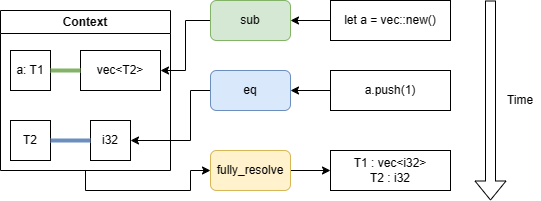
\includegraphics[width=120mm, height=45mm]{./img/RustTypeInference.png}
\caption{Rust type inference}
\label{img18:rustTypeInference}
\end{figure}
\par
\par
This global type inference is possible thanks to a type inference context which is shared across multiple statements. 
Figure \ref{img18:rustTypeInference} shows a basic principle how the the context works. 
It starts with an empty context. 
As the compiler traverses a method body, it adds new type variables that have to be solved and constrains them by the types which they are interacting with. 
The figure demonstrates it by adding a new type variable \texttt{T1} representing a type of the \texttt{a} variable.
It uses the \texttt{sub} function which adds the \texttt{Vec<T2>} subtyping constaint to the \texttt{T1} variable represented by a thick green line.
This constraint was obtained from a type of the initializing value \texttt{Vec::new()} which contains an unspecified type argument represented by a new \texttt{T2} type variable.
Since, the initializing type can't be fully resolved because the constraint contains the \texttt{T2} unbound type variable it has to postpone the resolution. 
It passes the context to binding the next statement, where it collects another constraint about the \texttt{T2} type argument of the initializing value.
The \texttt{sub} function is similar to the unification seen in the previous section \ref{sect03:HM}, where it extracts the required bounds of unbound type variables by finding substitutions for type variables in order to make matching types containing the type variables equal.
When there is enough information to resolve \texttt{T1} and \texttt{T2} type variables, they are resolved by finding an appropriate type for the type variable with respect to collected bounds.
In the given example, the bounds contain only one type, so the type variables are resolved to them.
\par
The mentioned sharing of context enables type inference to be backward, meaning that based on future type information, it is possible to infer already collected unbounded type variables. 
Besides sharing the context, there are other inference features that are missing in C\# type inference and would be valuable. 
The first of them is type inference in object creation expressions, which doesn't exist in C\#. 
The next regards collecting type constraints, which are obtained from a wider context than C\# uses. 
For example, If a generic method containing a type variable in the return type is used as an assignment of an already typed variable, the type variable is constrained by the type of the target. Other features regard the inner implementation of type inference, which offers probing to constrain a type variable without influencing the context. 
There is a possibility of a snapshot that records all changes and can be used for backtracking and finding the right inferred type arguments.
Although Rust type inference is more advanced in comparison with C\#, it has to be considered language differences making type inference computation cost and difficulty relative to their features. 
As an example, the overloading can mentioned causing exponetial time of type inference. 
Since Rust doesn't have overloading, the type inference can be more powerful without significant slowdown, which is not the case of C\# as will be shown in the following chapters.

\section{Github issues} \label{sect04:github}

The last section describes a process of proposing new C\# language features and mentions already existing ideas, presented in the C\# language repository, which will be an inspiration to the thesis's proposed improvement.
\par
The process of designing a new language feature starts with publishing an idea into discussions \cite{online:discussions}, where the C\# community can comment on it. 
The idea contains a brief description of the feature, motivation, and design. 
Besides the idea, a new language feature requires a proposal, initially published as an Github issue, describing the feature in a way that can be later reviewed by the \ac{LDM} committee.
If the proposal sufficiently merits the discussions, it can be marked as a \textit{champion} by a member of \ac{LDT} for being discussed further in \ac{LDM}. 
The state of a proposal is described by several milestones. 
The most important for the thesis is the \textit{AnyTime} milestone, meaning that the proposal is not actively worked on and is open to the community to collaborate on it. 
At the time of writing, a member of \ac{LDT} recommended championed issue \cite{online:champion} regarding \textit{partial type inference} to be investigated since it contains many related discussions with proposed changes but still doesn’t have a required proposal specification which would allow to be discussed by the team. 
When a proposal has sufficient quality to be discussed by \ac{LDT}, a member invites the proposer to make a \textit{pull request} where further collaboration continues. 
If \ac{LDT} accepts the proposal, it is added to the \textit{proposals} folder in the repository for being added into the C\# specification, and its future implementation (in Roslyn) will be shipped with the next C\# version. 
\par
The recommended issue doesn't contain a specific idea of the improvemenet rather the scope of the improvement.
The improvement suggests \textit{partial type inference} which would allow to hint ambigious type arguments which can't be inferred by a compiler instead of currently specifying the whole type argument list.
Since it doesn't have any concerete way how to achive it, there are presented related discussions directly or indirectly mentioned in the issue which partially suggest a possible solution.

\subsection{Default type parameters}

The first discussion \cite{online:DefTypeParam} mentions \textit{default type parameters} introducing default type arguments, which are used when explicit type arguments are not used. 
Figure \ref{img19:defTypeParam} shows a potential design of this feature where construing generic type \texttt{A} doesn’t need a type argument since it uses \texttt{int} type as a default value. 
\begin{figure}[h]
\begin{lstlisting}[style=csharp]
var temp = new A();

class A<T = int> {}
\end{lstlisting}
\caption{Default type parameters.}
\label{img19:defTypeParam}
\end{figure}

\subsection{Generic aliases}

The next discussion \cite{online:GenAlias} mentions \textit{generic aliases} allowing to specify default values similar to the goal of the previous discussion by defining an alias to that type with option generic parameters. 
Figure\ref{img20:genAlias} shows an example where there is the \texttt{StringDictionary} generic alias specifying the first type argument of the \texttt{Dictionary} class to be the \texttt{string} type, which simplifies the usage of the \texttt{Dictionary} type in scenarios where there are often used dictionaries with keys of the \texttt{string} type.
\begin{figure}[h]
\begin{lstlisting}[style=csharp]
var temp = new StringDictionary<int>();

using StringDictionary<TValue> = Dictionary<String, TValue>;
\end{lstlisting}
\caption{Generic aliases.}
\label{img20:genAlias}
\end{figure}

\subsection{Named type parameters}

Discussion \cite{online:NamedTypeParam} mentions \textit{named type parameters}, which are similar to named parameters of methods. 
The basic thought of this idea is being able to specify a type parameter for which an user provides a type argument by name. 
Figure \ref{img21:NamedTParam} shows a generic method \texttt{F} with two type parameters. 
The current type inference forces to specify all type arguments in the \texttt{F} method call since it is not able to infer the \texttt{U} type. 
Named type parameters offer a way how to tell the compiler specific type parameters for which an user provides type arguments, \texttt{U} in this case, and letting the compiler infer the rest of the type parameters.
\begin{figure}[h]
\begin{lstlisting}[style=csharp]
var x = F<U:short>(1);

U F<T, U>(T t) { ... }
\end{lstlisting}
\caption{Named type parameters.}
\label{img21:NamedTParam}
\end{figure}

\subsection{Inferred type argument}

Comments of the mentioned championed issue \cite{online:champion} propose several keywords that can be used in a type argument list for skipping type arguments, which can be inferred by the compiler and just providing the remaining ones. 
Figure \ref{img22:CharITArg} shows the \texttt{var} keyword for skipping the first type argument since it can be inferred from the argument list, and an user just specifies the second type argument, which can’t be inferred by the compiler. 
The comments propose other options for keywords like underscore or whitespaces.
\begin{figure}[h]
\begin{lstlisting}[style=csharp]
Foo<var, int>("string");

TResult Foo<T, TResult>(T p1){ ... }
\end{lstlisting}
\caption{Using char as inferred type argument.}
\label{img22:CharITArg}
\end{figure}

\subsection{Target-typed inference} \label{sect06:targetType}

Discussion \cite{online:RetTInference} proposes \textit{Target-typed inference}, where type inference uses type information of the target assigned by the return value. 
We can see the usage in Figure \ref{img62:RetTInf}, where type inference determines that the return type has to be \texttt{int} type and uses that to deduce the type argument \texttt{T}.
\begin{figure}[h]
\begin{lstlisting}[style=csharp]
object row = ...
int id = row.Field("id")

static class ObjectEx {
	T Field<T>(this object target, string fieldName) 
	{ ... }
}
\end{lstlisting}
\caption{Target-typed inference.}
\label{img62:RetTInf}
\end{figure}

\subsection{Type inference based on constrains}

The next idea of improving type inference is given by the discussion \cite{online:TInfConst}, where type inference utilizes type information obtained from type constraints.
A simple example of that can be seen in Figure \ref{img23:TInfConst}, where \texttt{T1} can be deduced by using \texttt{T1}'s constraint and inferred type of \texttt{T2} forming inferred type \texttt{List<int>}.
\begin{figure}[h!]
\begin{lstlisting}[style=csharp]
var temp = Foo(1);

T1 Foo<T1,T2>(T2 item) where T1 : List<T2> {}
\end{lstlisting}
\caption{Type inference based on type constraints.}
\label{img23:TInfConst}
\end{figure}

\subsection{Inferred method return type}

Discussion \cite{online:TMRetInf} mentions type inference of method return type known from the Kotlin programming language.
There is the usage in the following Figure \ref{img24:TMRetInf}, where the return type of the \texttt{Add} method is inferred to be \texttt{int} based on the type of the return expression.
\begin{figure}[h!]
\begin{lstlisting}[style=csharp]
public static Add(int x, int y ) => x + y;
\end{lstlisting}
\caption{Type inference of method return type.}
\label{img24:TMRetInf}
\end{figure}

\subsection{Realocation}

An issue \cite{online:Realloc} proposes a way to compact type argument lists of identifiers containing inner identifiers with argument lists. 
The idea is demonstrated in the example \ref{img25:Realloc}, where the argument list of \texttt{A<T1>} type and the \texttt{Foo<T2>} method are merged, and the type arguments are split by a semicolon.
\begin{figure}[h]
\begin{lstlisting}[style=csharp]
A.Foo<int;string>();

static class A<T1> {
    public static void Foo<T2>(){}
}
\end{lstlisting}
\caption{Specifying type arguments in method calls (Realocation).}
\label{img25:Realloc}
\end{figure}

\subsection{Constructor type inference}

The last discussion \cite{online:CtorTInf}, which is mentioned here, regards \textit{constructor type inference} enabling type inference for object creation expressions. 
The type inference can be seen in Figure \ref{img26:CtorTInf}, where the \texttt{T} type parameter of the \texttt{C<T>} generic type can be deduced by using type information from its constructor.
\begin{figure}[h]
\begin{lstlisting}[style=csharp]
var temp = new C<_>(1); // T = int

class C<T> { public C(T p1) {}}
\end{lstlisting}
\caption{Constructor type inference.}
\label{img26:CtorTInf}
\end{figure}
\chapter{Problem Analysis}

The previous section \ref{sect04:github} introduced the championed issue, accompanied by several ideas for the improvement.
Since the description of the issue is not well defined, the work will continue to set the scope of the issue, which will bound the proposed improvement of this thesis. 
In that scope, it will identify a concrete motivation that should be solved by the improvement and which would be a real-world missing feature, making the proposal promising to become a potential future extension of C\# language. 
Based on that motivation and information obtained from the previous sections, it will determine requirements that should be fulfilled by the improvement. 
The requirements will help to validate the thesis’s goals regarding the improvement.

\section{Scope}

The previous section \ref{sect05:mti}, regarding the method type inference, shows that type inference is a complicated process, where even the current C\# method type inference is difficult to understand. 
Hence, the thesis will choose a small part of C\# where it will improve and introduce the type inference and will be possible to reason about and implement in the scope of this text. 
The second reason for choosing a minor change is that introducing a completely new type inference in C\# would rather have an experimental result, which would have a smaller chance of getting into production. 
This consequence is different from the intention of this
work. 
However, some more extensive changes in the type inference will also be mentioned to outline possible obstacles to introducing them in the C\#.
\par
The thesis will focus on the already-mentioned \textit{partial type inference} proposal \ref{sect04:github}, which was recommended by a member of LDT and has a chance to be discussed in LDM and potentially accepted. 
Analysis of this improvement will contain a consideration of existing ideas, their consequences on C\#, and their difficulties in implementing them in Roslyn.

\section{Motivation} \label{sect10:mot}

Partial type inference focuses on hinting to the compiler ambiguous type arguments of generic type or method in situations where it can’t deduce them. 
In the context of C\#, the method type inference is the only type inference that infers type arguments. 
Even though the method type inference is a complex algorithm, it has several weaknesses. 
The following three real-world examples demonstrate common issues with the method type inference, which the thesis will try to solve.

\subsection{Weakness -- Target-typing}
The first weakness regards the target typing, which was mentioned in the previous chapter \ref{sect06:targetType}. 
Suppose a hypothetical situation when a user queries an item from a database whose column is a point of interest. 
Figure \ref{img27:usecase1} shows an example of code that uses the \texttt{fetch} method defined on a database type. 
The \texttt{data} variable represents data fetched from a database. 
Since a concrete form of data is unknown, the data has the type of \texttt{object} containing an internal representation of fetched data with the columns stored as fields. 
The \texttt{GetField} method enables to read the variable’s field of the given name with the supposed type given as a type argument. 
Suppose the fetched object contains the ``name'' field containing a string value. 
Now, a user wants to store the value in the \texttt{name} variable, which is explicitly typed. 
Even though the return type of the \texttt{GetField} method is known from the variable declaration, which is also the \texttt{TReturn} type argument of the method, the user still has to specify the type argument in the call. 
Generally, this problem consists of all type inferences, which depend on the target type. The target can be a parameter of another method call or an assigning field. 
If the method type inference considers the target type, the user will not have to specify the \texttt{string} type argument in the \texttt{GetField} call.
\begin{figure}[h]
\begin{lstlisting}[style=csharp]
TReturn GetField<TReturn>(object inst, string fieldName) { ... }
...
object data = database.fetch();
string name = GetField<string>(data, "name");
\end{lstlisting}
\caption{No target-typed inference.}
\label{img27:usecase1}
\end{figure}

\subsection{Weakness -- Constraints-based Inference}

The second weakness is noticeable in more advanced generic APIs, like testing frameworks, using type constraints containing the type parameters. 
Figure \ref{img28:usecase2} shows a scenario of a simple test framework that defines the \texttt{Test} method parameterized by a type of input data and a test case represented as type parameters \texttt{U} and \texttt{V}, respectively. 
The provided type argument representing the test case has to inherit the \texttt{TestCaseBase} base implementation, which is a generic type parametrized by a type of input data. 
\begin{figure}[h]
\begin{lstlisting}[style=csharp]
void Test<T, U>(U data) where T : TestCaseBase<U> { ... }
...
Test<TestCaseBase<MyData>, MyData>(new MyData());
\end{lstlisting}
\caption{No constraints-based inference.}
\label{img28:usecase2}
\end{figure}
This constraint gives type information about the \texttt{T} type parameter, which is related to the type of input data.
However, the user has to specify type arguments in the \texttt{Test} call since the type inference doesn’t consider this source of type information. 
If the compiler considers the constraint, the type arguments will be inferred because the constraint gives a lower bound of the first type argument and the second type argument can be inferred from the first argument of the method.

\subsection{Weakness -- All or Nothing Principle}

There are also situations where even strong type inference is not enough.
Figure \ref{img29:usecase3} shows a situation where the \texttt{Log} method is parametrized by two type parameters that are obtained in the parameter types and hence inferable by the compiler. 
However, the \texttt{Log} method call still has to specify type arguments because the \texttt{null} argument doesn’t have concrete type information. 
In this case, the user always has to specify the second type argument, but the compiler can infer the first type argument. 
The thesis refers to this problem as \textit{all or nothing} principle, which regards the obligation to specify all type arguments or none of them.
\begin{figure}[h]
\begin{lstlisting}[style=csharp]
void Log<T, U>(T message, U appendix) { ... }
...
Log<Message, Appendix>(new Message(...), null);
\end{lstlisting}
\caption{Uninferable type argument.}
\label{img29:usecase3}
\end{figure}

\subsection{Solution -- Improved Method Type Inference}

The first and the second weaknesses motivate us to extend the method type inference in order to consider a wider context for obtaining type information for the type arguments. 
This potential improvement is a problem for the compiler's backward compatibility which was mentioned in the C\# discussion \cite{online:breakingChange}. 
New compiler versions should be backward compatible so that a new version does not change the behavior of the code compiled by the older version.
\par
Figure \ref{img30:breakingChange1} shows the breaking change when the method type inference starts to consider target types.
\begin{figure}[h]
\begin{lstlisting}[style=csharp]
T M<T>(int p1) { ... }
int M(long p2) { ... }
...
int name = M(1);
\end{lstlisting}
\caption{Breaking change: Target-typed inference.}
\label{img30:breakingChange1}
\end{figure}
\par
Before the improvement, the \texttt{M} method call is resolved to the non-generic version of this method because type inference can’t infer the \texttt{T} type argument. 
After the improvement, the type inference infers \texttt{T} to be the \texttt{int} type, which is more specific to the type of \texttt{1} argument than the \texttt{long} type. 
So now, the \texttt{M} method call refers to the generic version of this method and executes different code without any warning or error.
\par
Figure \ref{img31:breakingChange2} shows a similar situation when the method type inference starts to consider type parameter constraints.
\begin{figure}[h]
\begin{lstlisting}[style=csharp]
void M<T>(int p1) where T : List<int> { ... }
void M(long p2) { ... }
...
M(1);
\end{lstlisting}
\caption{Breaking change: Constraints-based inference.}
\label{img31:breakingChange2}
\end{figure}
\par
Before the improvement, the \texttt{M} method call refers to the non-generic version of the method since the type inference can’t infer the type argument of a generic version. 
After the improvement, the generic version is inferred to have the \texttt{int} type argument and becomes to be more suitable for the overload resolution. 
So, the code behavior changed.
\par
Besides the breaking change, the potential method type inference improvement to use a bigger context still doesn’t solve our third weakness demonstrating a type parameter, which doesn’t appear in parameter types, the return type, and the type parameters’ constraints. 
These obstacles give the reason for introducing a way to hint just ambiguous type arguments to the compiler.

\subsection{Solution -- Partial Method Type Inference}

The partial method type inference can reduce the first two weaknesses. 
Type arguments, which the method type inference can’t infer, can be hinted in order to avoid specifying the whole type argument list. 
Let’s now ignore why the underscore character is used and how inferred type variables are determined in the following example. 
The reasons behind that will be mentioned later.
Figure \ref{img32:sol1} shows the usage of the partial method type inference applied in the second presented example regarding method type inference weaknesses. 
Although the first type argument of the \texttt{DoTest} method call must still be provided, the second argument is omitted by using the underscore character to determine an inferred type argument. 
The reduction of the first weakness is to isolate the insufficient type inference of type arguments that are directly influenced by it and to infer the rest.
\begin{figure}[h]
\begin{lstlisting}[style=csharp]
void DoTest<T, U>(U data) where T : TestCaseDefault<U> { ... }
...
DoTest<TestCaseDefault<MyData>, _>(new MyData());
\end{lstlisting}
\caption{Partial type inference: Reducing method type inference weakness.}
\label{img32:sol1}
\end{figure}
\par
The third motivation example confirms that the partial method type inference is not just a fix for missing type inference features but is needed when type arguments can’t be inferred at all. 
Figure \ref{img33:sol2} demonstrates a usage of the partial method type inference where it omits the first type argument since it can be deduced from the first argument type and specifies the ambiguous type that can’t be deduced.
\begin{figure}[h]
\begin{lstlisting}[style=csharp]
void Log<T, U>(T message, U appendix) { ... }
...
Log<_, Appendix>(new Message(...), null);
\end{lstlisting}
\caption{Partial type inference: Solving the \textit{all or nothing} problem.}
\label{img33:sol2}
\end{figure}

\newpage

\subsection{Solution -- Constructor Type Inference}

The partial type inference doesn’t regard only the partial method type inference. 
It can also be introduced in other places. One of the places that seems to be good for that is object creation expression. 
Except for the already mentioned \texttt{new()} operator, no other type inference infers type arguments of a construing generic type. The usage of the type inference is limited since the \texttt{new()} operator requires a target type to infer the construing type. 
Figure \ref{img34:wrapper} shows an example of the limitation, where the \texttt{new()} operator can’t be used since the \texttt{IWrapper} target type is not the \texttt{Wrapper<int>} construing type. 
Hence, the user has to specify the type with the \texttt{int} type argument, despite the fact that it could be inferred using the method type inference algorithm adjusted to be used in the object creation expression binding.
\begin{figure}[h]
\begin{lstlisting}[style=csharp]
class Wrapper<T> : IWrapper { public Wrapper(T item) { ... } }
...
IWrapper a = new Wrapper<int>(1);
\end{lstlisting}
\caption{C\# wrapper class.}
\label{img34:wrapper}
\end{figure}
\par
Generally, the object creation can be considered a special case of a method call with a side effect(creating the object), which already has the method type inference. 
Figure \ref{img35:workaroung} shows a workaround using the \texttt{Create} method, delegating the creation to the constructor call. 
\begin{figure}[h!]
\begin{lstlisting}[style=csharp]
static Wrapper<T> Create<T>(T item) => new Wrapper<T>(item);
...
IWrapper a = Create(1);
\end{lstlisting}
\caption{Workaround of constructor type inference.}
\label{img35:workaroung}
\end{figure}
Since the method call type arguments can be inferred, it allows the use of the method type inference for inferring type arguments of construing type. 
However, this solution has disadvantages like the necessary boiler-plate and a prohibition of using initializers.
\par
A possible solution would be to use the method type inference in object creation expression. 
Although this solution would be simple to implement, class type parameters are more likely not to be used in constructor parameter types, which makes the method type inference useless. 
Besides that, options for inferring type arguments of the construing type are not limited by not introducing breaking changes since there is no type inference at all now. 
So, there is a possibility of introducing an even stronger type inference, which could be one day introduced in the method type inference when there would be a way to make breaking changes in the new compiler version. 
\par
Figure \ref{img36:cti} shows an example of such a generic class whose all type parameters are not used in the constructor.
\begin{figure}[h]
\begin{lstlisting}[style=csharp]
class Algorithm<TData, TLogger> where TLogger : Logger<TData> 
{ public Algorithm(TData data) { ... } }
\end{lstlisting}
\caption{Use case using type parameter constraints.}
\label{img36:cti}
\end{figure}
\newpage
Because of that, extending the potential method type inference algorithm to be used in object creation expressions would be useless since the \texttt{TLogger} can’t be inferred only from parameter types.
\par
Introducing improved type inference based on the method type inference algorithm would solve the mentioned issues. 
Figure \ref{img37:sol1} shows a potential usage of that type inference in the first case regarding the \texttt{Wrapper} class where an underscore is used to represent an inferred type argument. 
The inference uses the parameter type of the constructor to infer the \texttt{T} parameter type which is \texttt{int}.
\begin{figure}[h]
\begin{lstlisting}[style=csharp]
class Wrapper<T> : IWrapper { public Wrapper(T item) { ... } }
...
IWrapper a = new Wrapper<_>(1);
\end{lstlisting}
\caption{Constructor type inference: Wrapper.}
\label{img37:sol1}
\end{figure}
\par
Figure \ref{img38:sol2} shows a potential extension of the type inference. 
There is the \texttt{Algorithm} class definition containing two type parameters representing the type of data and logger used by the class.
The first statement of initializing the \texttt{alg} variable uses type inference, leveraging the \texttt{TLogger}’s constraint to determine its type.
Now imagine that there is the \texttt{SpecialLogger} class that is intended to be used as a logger.
The second statement demonstrates the possibility of having a nested underscore, which allows to specify the type of logger without providing its type argument.
\begin{figure}[h]
\begin{lstlisting}[style=csharp]
class Algorithm<TData, TLogger> where TLogger : Logger<TData> 
{ public Algorithm(TData data) { ... } }
...
var alg = new Algorithm<_, _>(new MyData());
var algWithSpecialLogger = 
  new Algorithm<_ , SpecialLogger<_>>(new MyData());
\end{lstlisting}
\caption{Constructor type inference: stronger method type inference.}
\label{img38:sol2}
\end{figure}
\par
From now on, thesis calls \textit{constructor type inference} for introducing such a type inference.

\section{Requirements}

The following requirements should be fulfilled by the solution to make it more likely to be discussed by LDT.
\par
\textbf{Backward compatibility} is one of the most important requirements for new language features. 
The improvement shouldn’t introduce a breaking change. However, this requirement is sometimes too strict for improvements, which would be very beneficial, and its breaking change would appear in cases that seem to be rare in the code. 
These improvements can break backward compatibility by providing additional warnings or errors alerting a user of possible code behavior changes.
Figure \ref{img39:brkCh} shows an introduced breaking change when record classes were added into the C\# language. 
Before the change, the \texttt{B} identifier referred to a method without parameters and returned the type named \texttt{record}. 
After the change, the \texttt{B} identifier refers to a new record type declaration. 
There is an example where the breaking change can appear when there is a type with the \texttt{record} name. 
These situations are uncommon, and the improvement benefit was big enough to be added to the language. 
The possible breaking change is notified to the user by a compilation error.
\begin{figure}[h]
\begin{lstlisting}[style=csharp]
class record {}
class A {
  record B() { ... }
}
\end{lstlisting}
\caption{C\# record class breaking change.}
\label{img39:brkCh}
\end{figure}
\par
\textbf{Convenience} is a key requirement to make the improvement useful. 
Regarding the partial type inference, the improvement should propose a convenient way to skip ambiguous type arguments. 
The way should also be possible to use in different places where skipping type arguments could yield an advantage, like the type variable declaration or casting to a different type. 
The constructor type inference should be advanced enough to cover the mentioned examples in the previous section.
\par
\textbf{Extensibility} would make the improvement open for new features that can be needed in future language versions. 
The improvement should consider possible future improvements and not be a blocker for them.
\par
\textbf{Performance} is a critical part of Roslyn and which is one of the main goals of this project.
The time complexity added by the thesis’s improvement shouldn’t be too big in order to not slow the compilation process.

\section{Summary}

Three possible improvements of type inference were introduced based on the mentioned motivation, where was identified main weaknesses of the current type inference. 
Then, several requirements were created to achieve the fourth goal of the thesis, which is to make the proposal likely to be discussed by LDT. 
Based on the requirements, the first improvement introducing breaking change was excluded. 
The remaining two improvements seem to fulfill the requirements, and they will be further proceeded in the following section with focusing on not breaking any mentioned requirements.
\chapter{Solution}

\section{Proposal}

\section{Implementation}

\change{Describe process of making proposal and the prototype.}
\change{Describe partial method type inference.}
\change{Describe constructor type inference.}
\change{Describe generic adjusted algorithm for type inference.}
\change{Describe decisions of proposed change design.}
\change{Describe changed parts of C\# standard.}
\chapter{Evaluation}

\change{Describe achieved type inference. Mention interesting capabilities.}
\change{Note about the performance.}
\change{Links to csharplang discussions.}
\chapter{Future improvements}

\change{Mention next steps which can be done.}
\change{Discuss which steps would not be the right way(used observed difficulties).}

\chapter*{Conclusion}
\addcontentsline{toc}{chapter}{Conclusion}

The introduction \ref{sect:summary} sets four goals, which are gradually achieved by the thesis. 
It starts by exploring C\# type inference by using the language specification and implementation in the Roslyn project. 
Then, it compares with Rust type inference, which offers more advanced type inference than C\#. 
These differences are explained using the theory background of Hindley-Milner type inference, which describes the limits of type inference in strongly typed languages.
\par
Based on these observations, the work selects a subset of type inference improvements suggested in C\# language discussions on GitHub and explores the motivation behind it to make it likely to add to C\# language. 
The motivation is described in the created proposal, which is the fourth goal and which describes the improvement in terms of changing the specification.
\par
Together with the proposal, the implementation was made in the Roslyn project fork, with unit tests checking the functionality. 
This was the last goal of the proposal. 
The implementation ensured that basic compiler tests passed to reveal possible issues with the solution.
\par
In addition to the mentioned goals, the thesis succeeded in presenting the proposal and implementation to the \ac{LDM} responsible for approving language changes into C\#. 
The committee agreed to continue with the change for further discussion and is generally inclined to ship it with future language releases.
\par
Based on the goals achieved and additional success in the \ac{LDM} meeting, which was not a part of the scope of the work, we think that the thesis accomplished all the promised goals.


%%% Bibliography
%%% Bibliography (literature used as a source)
%%%
%%% We employ bibTeX to construct the bibliography. It processes
%%% citations in the text (e.g., the \cite{...} macro) and looks up
%%% relevant entries in the bibliography.bib file.
%%%
%%% The \bibliographystyle command selects, which style will be used
%%% for references from the text. The argument in curly brackets is
%%% the name of the corresponding style file (*.bst). Both styles
%%% mentioned in this template are included in LaTeX distributions.

\bibliographystyle{plainnat}    %% Author (year)
% \bibliographystyle{unsrt}     %% [number]

\renewcommand{\bibname}{Bibliography}

%%% Generate the bibliography. Beware that if you cited no works,
%%% the empty list will be omitted completely.

\bibliography{bibliography}

%%% If case you prefer to write the bibliography manually (without bibTeX),
%%% you can use the following. Please follow the ISO 690 standard and
%%% citation conventions of your field of research.

% \begin{thebibliography}{99}
%
% \bibitem{lamport94}
%   {\sc Lamport,} Leslie.
%   \emph{\LaTeX: A Document Preparation System}.
%   2nd edition.
%   Massachusetts: Addison Wesley, 1994.
%   ISBN 0-201-52983-1.
%
% \end{thebibliography}


%%% Figures used in the thesis (consider if this is needed)
\listoffigures

%%% Tables used in the thesis (consider if this is needed)
%%% In mathematical theses, it could be better to move the list of tables to the beginning of the thesis.
\listoftables

%%% Abbreviations used in the thesis, if any, including their explanation
%%% In mathematical theses, it could be better to move the list of abbreviations to the beginning of the thesis.
\chapwithtoc{List of Abbreviations}
\begin{acronym}
 \acro{LDT}{Language Design Team}
 \acro{LDM}{Language Design Meetings}
 \acro{AST}{Abstract Syntax Tree}
 \acro{CIL}{Common Intermediate Language}
\end{acronym}

%%% Attachments to the master thesis, if any. Each attachment must be
%%% referred to at least once from the text of the thesis. Attachments
%%% are numbered.
%%%
%%% The printed version should preferably contain attachments, which can be
%%% read (additional tables and charts, supplementary text, examples of
%%% program output, etc.). The electronic version is more suited for attachments
%%% which will likely be used in an electronic form rather than read (program
%%% source code, data files, interactive charts, etc.). Electronic attachments
%%% should be uploaded to SIS and optionally also included in the thesis on a~CD/DVD.
%%% Allowed file formats are specified in provision of the rector no. 72/2017.
\appendix
\chapter{Attachments}

\openright
\end{document}
